% ====chapter=====
\myChapter{Approche proposée pour la génération d'applications web pilotées par BPMN}{Approche proposée}
\label{chap:approche-prooweb}
\myMiniToc{mysection}{Sommaire}

\mySection{Introduction}{}

Les chapitres précédents ont permis de clarifier les notions mobilisées dans ce travail et de mettre en évidence les limites des travaux existants. BPMN offre un langage solide pour représenter le déroulement d'un processus métier, mais il ne suffit pas à décrire, à lui seul, toutes les informations nécessaires à la production d'une application web complète. La démarche proposée dans ce chapitre part de ce constat. Elle présente une approche d'ingénierie qui associe un modèle BPMN standard à une spécification applicative complémentaire afin de générer les principaux artefacts d'une application web orientée processus. L'objectif n'est pas seulement d'automatiser une partie du développement, mais de conserver un lien clair entre le processus métier, les règles d'accès, les données manipulées, les interfaces proposées aux utilisateurs et le code produit. Ce chapitre décrit ainsi le positionnement méthodologique de l'approche, l'architecture du framework, le modèle d'entrée enrichi, les règles de transformation retenues et le mécanisme prévu pour préserver les ajouts manuels du développeur.

\mySection{Vue d'ensemble de l'approche}{}

L'approche proposée relève de l'ingénierie dirigée par les modèles. Elle reprend l'idée centrale de la Model-Driven Architecture : partir d'un modèle métier, le transformer en modèle plus proche de la plateforme, puis produire des artefacts logiciels \cite{omg2014mda,jezequel2012}. Dans notre cas, le modèle métier est le diagramme BPMN 2.0. Il décrit la logique du processus, les activités, les passerelles, les événements et les flux d'enchaînement \cite{omg2013bpmn}.

Le BPMN ne porte cependant pas toutes les informations attendues par une application web. Il ne précise pas toujours les champs d'un formulaire, les rôles autorisés, les sources de données, les règles de visibilité ou les structures de persistance. Pour combler cette limite sans dénaturer le diagramme, l'approche associe au fichier BPMN une spécification applicative appelée \textit{spec-v1}. Le BPMN reste donc le support de la logique métier, tandis que \textit{spec-v1} décrit les informations nécessaires à la génération.

La chaîne retenue est volontairement courte : le BPMN et \textit{spec-v1} sont lus, validés, fusionnés dans un modèle applicatif intermédiaire, puis projetés vers le code. Ce modèle intermédiaire joue le rôle de PSM : il contient les activités qualifiées, les rôles, les entrées, les sorties, les règles de visibilité, les données partagées et les artefacts à produire. La génération modèle-à-texte s'appuie ensuite sur ce modèle stabilisé pour produire les fichiers de l'application \cite{syriani2018}.

Cette organisation répond à une exigence simple : ne pas demander au générateur de deviner. Toute information utile doit être présente dans le BPMN, dans \textit{spec-v1} ou dans une configuration prévue. Cette contrainte rend l'approche plus rigoureuse, car elle limite les interprétations implicites et facilite la traçabilité entre le processus modélisé et le code généré.

\mySection{Architecture globale du framework proposé}{}

L'architecture globale de ProOWeb est organisée autour d'une chaîne de génération qui va du modèle de processus vers une application web exploitable. Elle distingue clairement l'environnement de préparation des modèles, le coeur de transformation et l'espace de production des artefacts. Cette séparation est importante, car ProOWeb n'est pas seulement une application générée : il s'agit d'un framework qui prépare, contrôle et produit d'autres applications à partir d'un modèle BPMN enrichi. La figure \ref{fig:chap3-architecture-prooweb} présente cette organisation générale.

\begin{figure}[H]
\centering
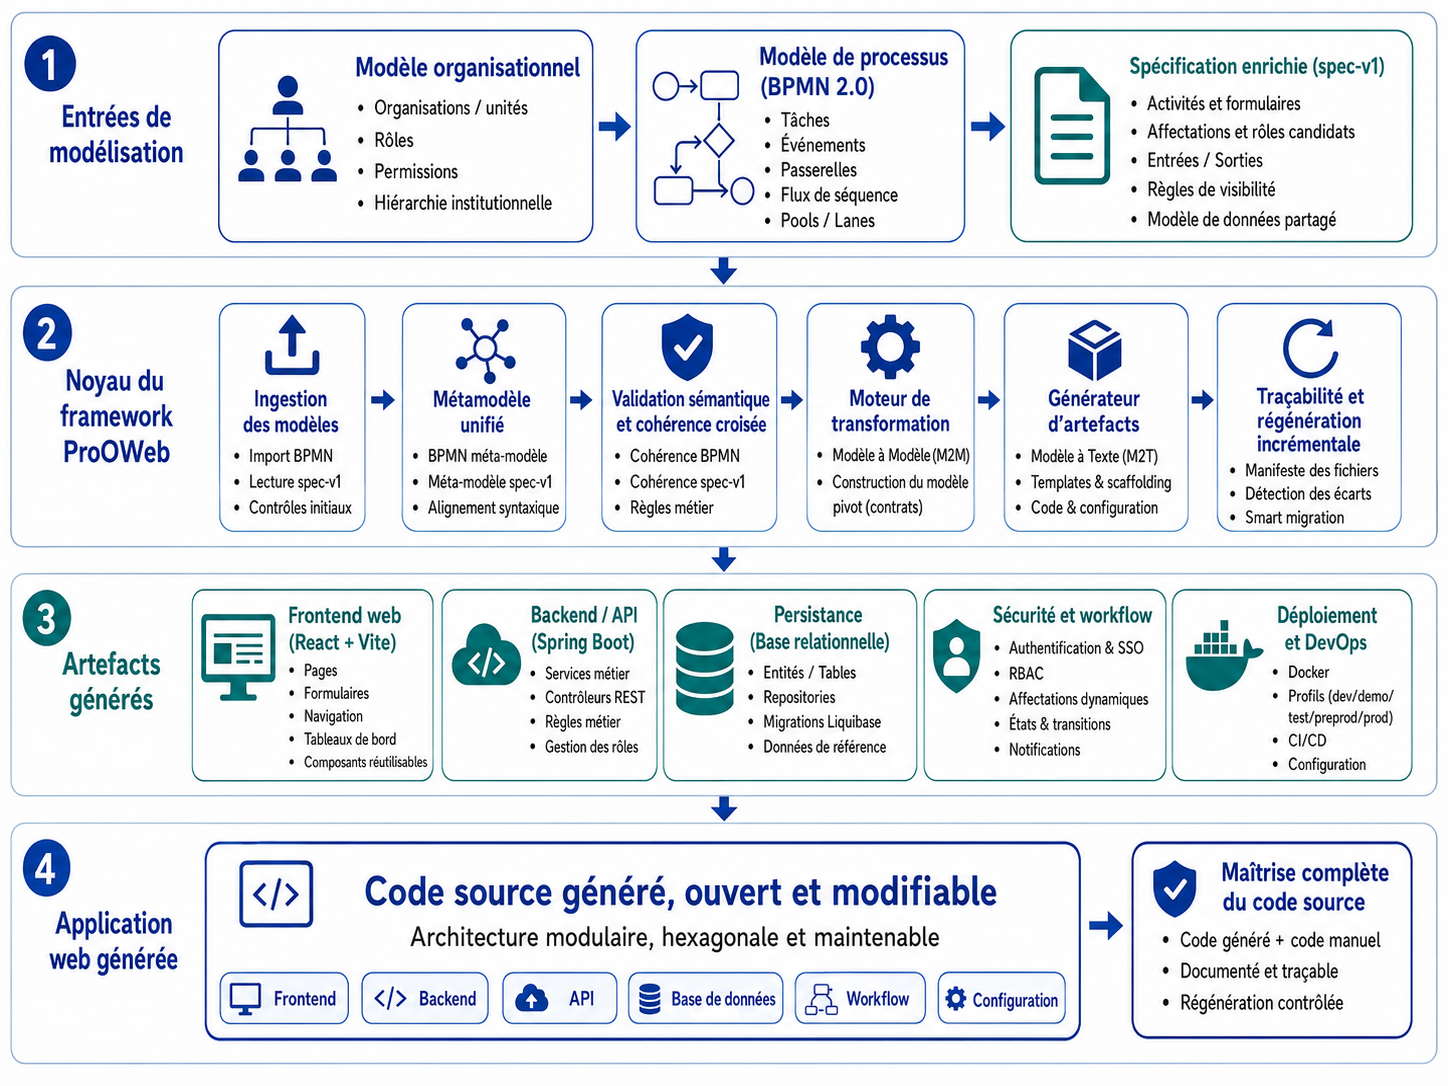
\includegraphics[width=0.80\textwidth]{Chap3/images/architecture_ProOWeb1.png}
\caption{Architecture de ProOWeb}
\label{fig:chap3-architecture-prooweb}
\end{figure}

\subsection{Architecture fonctionnelle du framework}

La figure \ref{fig:chap3-architecture-prooweb} met en évidence les principaux composants fonctionnels de ProOWeb. Chaque composant intervient à un moment précis de la chaîne et porte une responsabilité identifiable. L'intérêt de cette organisation est d'éviter que la génération soit concentrée dans un seul mécanisme opaque. Le modèle BPMN est d'abord interprété, la spécification \textit{spec-v1} est ensuite rapprochée du processus, les contrats intermédiaires sont construits, puis les artefacts logiciels sont produits à partir de gabarits.

Cette architecture adopte une logique progressive. Le sous-système d'ingestion prépare le workflow. Le module d'enrichissement donne une signification applicative aux activités. Le noyau de transformation modèle-à-modèle produit les contrats intermédiaires. Le moteur de génération modèle-à-texte matérialise ces contrats dans le projet cible. À ces composants s'ajoutent des fonctions transversales de validation, de gestion des versions, de suivi des fichiers générés et de production de rapports.

\subsubsection{Sous-système d'ingestion du modèle BPMN}

Le sous-système d'ingestion du modèle BPMN constitue le point d'entrée métier de ProOWeb. Sa fonction est de prendre en charge le modèle de processus, qu'il provienne d'une modélisation réalisée dans l'environnement du framework ou d'un fichier BPMN déjà existant. À ce niveau, ProOWeb ne cherche pas encore à produire du code. Il prépare une représentation exploitable du workflow.

Le sous-système d'ingestion extrait les éléments structurants du fichier BPMN : identifiant du processus, activités, événements, passerelles, flux de séquence, activités initiales et activités terminales. Il reconstitue également les liens entrants et sortants de chaque activité. Cette reconstruction est nécessaire pour déterminer comment une instance de processus pourra progresser dans l'application générée.

La représentation produite par le sous-système d'ingestion sert de base aux traitements suivants. Lorsqu'une passerelle est rencontrée, ProOWeb isole le point de décision afin que la règle correspondante puisse être validée ou complétée dans \textit{spec-v1}. Lorsqu'une activité est détectée, son identifiant devient une référence utilisée par la spécification enrichie. Cette contrainte empêche la dissociation entre le diagramme BPMN et les règles applicatives qui lui sont associées.

\subsubsection{Module d'enrichissement à partir de la spécification}

Le module d'enrichissement à partir de la spécification relie le workflow BPMN aux informations applicatives décrites dans \textit{spec-v1}. Son rôle est décisif, car le BPMN indique le déroulement du processus mais ne contient pas tous les éléments nécessaires à une application web. Le module d'enrichissement associe donc, à chaque activité concernée, son type, ses rôles candidats, sa stratégie d'affectation, ses sources d'entrée, ses sorties, sa stratégie de stockage et ses règles de visibilité.

Le module d'enrichissement réalise aussi un premier contrôle de cohérence. Une activité déclarée dans \textit{spec-v1} doit correspondre à un identifiant présent dans le modèle BPMN. Une activité manuelle doit disposer d'informations suffisantes pour être traitée par un utilisateur. Une activité automatique doit indiquer le comportement attendu ou le gestionnaire à invoquer. Ces contrôles évitent de reporter dans les templates de génération des décisions qui doivent être résolues avant la production du code.

Grâce à l'enrichissement, une tâche BPMN cesse d'être seulement une étape graphique du processus. Elle devient une unité applicative capable de produire une vue de traitement, une règle d'affectation, un point d'entrée back-end, une transition de runtime et éventuellement une opération de persistance. C'est à ce niveau que le processus commence à prendre la forme d'une application.

\subsubsection{Noyau de transformation modèle-à-modèle}

Le noyau de transformation modèle-à-modèle assure la construction du modèle pivot de ProOWeb. Il prend en entrée la représentation BPMN préparée par le sous-système d'ingestion et les informations applicatives fournies par le module d'enrichissement. À partir de ces deux sources, il produit des contrats intermédiaires qui structurent l'application à générer. Cette démarche rejoint le principe des transformations de modèles, qui consistent à établir des correspondances explicites entre des concepts sources et des concepts cibles \cite{omgqvt}.

Le noyau de transformation modèle-à-modèle produit notamment le \textit{runtime contract}, le \textit{data contract}, les catalogues destinés au front-end et le registre des processus générés. Le \textit{runtime contract} décrit les activités, les transitions, les rôles autorisés à démarrer une instance, les rôles de supervision et les règles liées à l'exécution. Le \textit{data contract} décrit les sources de données, les mappings de sortie, les stratégies de stockage et le lignage des informations. Les catalogues front-end exposent les métadonnées nécessaires aux vues et aux formulaires.

Le noyau de transformation modèle-à-modèle joue également un rôle de sécurisation de la génération. Il vérifie qu'une activité enrichie existe dans le BPMN, qu'une activité manuelle possède des rôles d'exécution, qu'une donnée produite possède une destination et qu'une source déclarée peut être résolue. Lorsque ces conditions ne sont pas remplies, ProOWeb doit produire un diagnostic clair plutôt qu'un code incertain. La génération devient ainsi contrôlable et vérifiable.

\subsubsection{Moteur de génération modèle-à-texte}

Le moteur de génération modèle-à-texte constitue la partie productive de ProOWeb. Il reçoit les contrats intermédiaires validés et applique les templates correspondant aux technologies cibles. Les templates back-end produisent les fichiers Spring Boot, les contrôleurs, les services, les ports, les adaptateurs, les configurations et les tests. Les templates front-end produisent les modules React/Vite, les catalogues de processus, les composants de traitement et les vues de supervision. Les templates de déploiement peuvent produire les fichiers Docker, les scripts et les profils d'exécution.

Le moteur de génération modèle-à-texte ne doit pas porter seul la logique de décision. Les décisions principales doivent déjà être stabilisées dans les contrats intermédiaires. Les templates ont alors pour fonction de matérialiser ces décisions dans les fichiers du projet cible. Cette séparation améliore la maintenabilité de la chaîne de génération \cite{syriani2018}.

Le moteur de génération modèle-à-texte participe enfin à la gouvernance du code produit. Chaque fichier généré peut être suivi dans le manifeste \texttt{.prooweb-managed.json}, avec son chemin, sa catégorie, ses propriétaires et son empreinte. Ce suivi prépare la migration intelligente : lors d'une nouvelle génération, ProOWeb peut identifier les fichiers maîtrisés par le générateur, détecter les modifications manuelles et produire un rapport de régénération.

\begin{table}[H]
\centering
\small
\caption{Rôle des composants fonctionnels du framework}
\label{tab:chap3-composants-framework}
\begin{tabular}{p{3.4cm}p{4.4cm}p{6.2cm}}
\hline
\textbf{Composant fonctionnel} & \textbf{Entrée principale} & \textbf{Résultat attendu} \\
\hline
Sous-système d'ingestion BPMN & Fichier BPMN XML ou modèle édité & Représentation interne du workflow, activités, transitions et points de décision. \\
Module d'enrichissement applicatif & Spécification \textit{spec-v1} & Activités qualifiées, rôles, affectations, données, sorties et visibilité. \\
Noyau de transformation M2M & Workflow interprété et enrichissements validés & Contrats intermédiaires : \textit{runtime contract}, \textit{data contract}, catalogues et registre. \\
Moteur de génération M2T & Contrats intermédiaires & Artefacts Spring Boot, React/Vite, persistance, configuration, scripts et rapports. \\
\hline
\end{tabular}
\end{table}

\mySection{Modèle d'entrée enrichi : spécification spec-v1}{}

La spécification \textit{spec-v1} constitue le complément applicatif du modèle BPMN. Elle ne remplace pas le diagramme de processus ; elle lui ajoute les informations nécessaires pour produire une application web orientée processus. Son rôle est donc de rendre explicites les décisions qui ne sont pas naturellement portées par BPMN : démarrage d'une instance, supervision, affectation des tâches, sources d'entrée, sorties, visibilité, données partagées et comportement des activités automatiques.

Dans ProOWeb, \textit{spec-v1} est attachée à une version de modèle de processus. Elle participe ainsi au même cycle de préparation que le BPMN : rédaction, validation, simulation, promotion et déploiement. Cette organisation évite qu'un processus soit généré à partir d'un diagramme validé mais d'une spécification incomplète. La spécification devient une partie du modèle d'entrée, au même titre que le fichier BPMN.

\subsection{Structure générale de la spécification}

La structure générale de \textit{spec-v1} est organisée autour de rubriques fonctionnelles. La rubrique de démarrage précise les rôles autorisés à lancer une instance et les activités initiales. La rubrique de supervision indique les rôles capables de suivre ou d'administrer un processus. La rubrique des activités décrit chaque étape BPMN à enrichir. La rubrique des données partagées définit les entités persistantes manipulées par l'application au-delà d'une instance particulière.

La spécification utilise également des valeurs contrôlées. Les types d'activités sont par exemple limités à des catégories comme \texttt{MANUAL} et \texttt{AUTOMATIC}. Les stratégies d'affectation appartiennent à une liste connue. Les sources de données et les stratégies de stockage sont aussi normalisées. Cette discipline réduit les ambiguïtés et rend la génération plus prévisible.

\begin{lstlisting}[caption={Structure simplifiée de la spécification spec-v1},label={lst:chap3-structure-specv1}]
{
  "processId": "processus_demande",
  "schemaVersion": 1,
  "start": {
    "allowedRoles": ["DEMANDEUR"],
    "startActivities": ["saisir_demande"]
  },
  "monitoring": {
    "supervisorRoles": ["SUPERVISEUR", "ADMINISTRATEUR"]
  },
  "activities": {
    "saisir_demande": {
      "activityType": "MANUAL",
      "assignment": {},
      "input": {},
      "output": {},
      "visibility": {}
    }
  },
  "sharedData": {
    "entities": []
  }
}
\end{lstlisting}

Cette structure montre que \textit{spec-v1} ne se limite pas à un catalogue de formulaires. Elle décrit les conditions de démarrage, les rôles de supervision, la qualification des activités et le modèle de données partagé. Les informations ainsi déclarées alimentent ensuite le \textit{runtime contract}, le \textit{data contract}, les catalogues front-end et les artefacts générés.

Une activité enrichie décrit la manière dont une étape BPMN devient une unité applicative. L'extrait suivant illustre une tâche manuelle. Les champs présentés n'ajoutent pas une nouvelle notation métier ; ils indiquent ce dont le framework a besoin pour construire les contrats intermédiaires et générer les artefacts correspondants.

\begin{lstlisting}[caption={Extrait schématique d'une activité enrichie},label={lst:chap3-activite-enrichie}]
"valider_demande": {
  "activityType": "MANUAL",
  "assignment": {
    "candidateRoles": ["VALIDATEUR"],
    "mode": "CLAIM",
    "strategy": "ROLE_BASED"
  },
  "input": {
    "sources": ["PROCESS_CONTEXT", "PREVIOUS_ACTIVITY"]
  },
  "output": {
    "storage": "BOTH",
    "mappings": []
  },
  "visibility": {
    "activityViewerRoles": ["VALIDATEUR", "SUPERVISEUR"],
    "dataViewerRoles": ["VALIDATEUR"]
  }
}
\end{lstlisting}

Cet extrait rend visible le passage du processus vers l'application. L'identifiant \texttt{valider\_demande} renvoie à une activité BPMN. La propriété \texttt{activityType} indique la nature de l'activité. La section \texttt{assignment} oriente l'affectation de la tâche. Les sections \texttt{input} et \texttt{output} organisent les données. La section \texttt{visibility} distingue les rôles qui peuvent voir l'activité de ceux qui peuvent consulter les données associées.

\subsection{Métadonnées des activités}

Les métadonnées des activités précisent la manière dont chaque étape du processus doit être prise en charge dans l'application. La propriété \texttt{activityType} distingue les activités manuelles des activités automatiques. Une activité manuelle est destinée à être traitée par un utilisateur. Elle doit donc être reliée à des rôles candidats, à une politique d'affectation, à des données visibles et à des sorties attendues. Une activité automatique est exécutée par le système. Elle peut alors être associée à un gestionnaire, à un type de tâche automatique, à un mode de déclenchement et à une configuration.

Cette distinction structure la génération. Une activité manuelle peut conduire à une vue de traitement, à une entrée dans la liste des tâches, à une route de complétion et à une règle d'autorisation. Une activité automatique peut conduire à un service applicatif, à un adaptateur ou à un appel interne. Le générateur ne traite donc pas toutes les activités de manière uniforme ; il applique une projection différente selon la nature déclarée dans \textit{spec-v1}.

\subsection{Affectation des tâches et sécurité}

L'affectation des tâches est l'un des points les plus sensibles d'une application orientée processus. Une tâche manuelle doit être visible ou attribuée aux bons utilisateurs. Dans \textit{spec-v1}, cette dimension est décrite à travers les rôles candidats, le mode d'affectation, la stratégie retenue et, si nécessaire, les rôles autorisés à réaliser une affectation manuelle.

Plusieurs stratégies peuvent être prises en charge. \texttt{ROLE\_QUEUE} rend une tâche accessible aux utilisateurs possédant les rôles candidats. \texttt{SUPERVISOR\_ONLY} l'oriente vers un superviseur. \texttt{SUPERVISOR\_THEN\_ANCESTORS} remonte la hiérarchie si nécessaire. \texttt{UNIT\_MEMBERS} exploite l'appartenance organisationnelle. \texttt{SINGLE\_MATCH\_ONLY} exige une résolution non ambiguë. \texttt{MANUAL\_ONLY} impose une affectation explicite. \texttt{ROUND\_ROBIN} répartit les tâches entre plusieurs candidats.

Ces règles sont liées à la sécurité. L'authentification peut être interne ou confiée à un fournisseur externe, mais l'autorisation applicative reste portée par les rôles du système généré. Les recommandations de l'OWASP rappellent l'importance de contrôler les accès et de limiter l'exposition des fonctionnalités sensibles \cite{owaspTopTen2026}. Dans ProOWeb, les rôles déclarés dans \textit{spec-v1} alimentent donc les contrôles côté back-end et les adaptations d'affichage côté front-end.

\begin{table}[H]
\centering
\small
\caption{Stratégies d'affectation prises en charge dans la spécification}
\label{tab:chap3-strategies-affectation}
\begin{tabular}{p{4.4cm}p{9.5cm}}
\hline
\textbf{Stratégie} & \textbf{Interprétation dans ProOWeb} \\
\hline
\texttt{ROLE\_QUEUE} & Rend la tâche disponible aux utilisateurs possédant les rôles candidats déclarés. \\
\texttt{SUPERVISOR\_ONLY} & Oriente la tâche vers le superviseur associé au contexte organisationnel. \\
\texttt{SUPERVISOR\_THEN\_ANCESTORS} & Recherche un superviseur, puis remonte la hiérarchie lorsque le premier niveau ne suffit pas. \\
\texttt{UNIT\_MEMBERS} & Rend la tâche accessible aux membres d'une unité organisationnelle. \\
\texttt{SINGLE\_MATCH\_ONLY} & Autorise l'affectation automatique uniquement lorsqu'un seul candidat correspond. \\
\texttt{MANUAL\_ONLY} & Exige une intervention explicite d'un utilisateur autorisé à affecter. \\
\texttt{ROUND\_ROBIN} & Répartit les tâches de manière déterministe entre plusieurs candidats. \\
\hline
\end{tabular}
\end{table}

\subsection{Gestion des entrées et sorties de données}

La gestion des entrées et sorties transforme une activité BPMN en opération applicative. Une activité peut lire des données provenant du contexte du processus, d'une activité précédente, d'un espace de données partagées, d'un service back-end ou d'un service externe. Ces sources sont représentées par des valeurs contrôlées afin que le générateur sache comment résoudre les données au moment de l'exécution.

La propriété \texttt{input.sources} indique l'origine des informations nécessaires à l'activité. Les valeurs \texttt{PROCESS\_CONTEXT}, \texttt{PREVIOUS\_ACTIVITY}, \texttt{SHARED\_DATA}, \texttt{BACKEND\_SERVICE} et \texttt{EXTERNAL\_SERVICE} expriment respectivement le contexte de l'instance, les résultats d'une activité antérieure, les données métier partagées, un service interne ou un service externe.

La propriété \texttt{output.storage} précise la destination des données produites. La valeur \texttt{INSTANCE} conserve la sortie dans l'état de l'instance. La valeur \texttt{SHARED} projette la sortie vers les données partagées. La valeur \texttt{BOTH} maintient la donnée dans les deux espaces. Les mappings de sortie indiquent ensuite comment les champs produits par l'activité sont projetés vers les structures persistantes.

\begin{table}[H]
\centering
\small
\caption{Interprétation des principales sources de données}
\label{tab:chap3-sources-donnees}
\begin{tabular}{p{4.2cm}p{9.6cm}}
\hline
\textbf{Source} & \textbf{Interprétation dans la génération} \\
\hline
\texttt{PROCESS\_CONTEXT} & Données générales liées à l'instance du processus, comme son identifiant, son état ou certains paramètres globaux. \\
\texttt{PREVIOUS\_ACTIVITY} & Données produites par une activité antérieure et nécessaires à l'activité courante. \\
\texttt{SHARED\_DATA} & Données métier persistantes, représentées par des entités partagées dans l'application. \\
\texttt{BACKEND\_SERVICE} & Données obtenues par un service interne de l'application générée. \\
\texttt{EXTERNAL\_SERVICE} & Données récupérées auprès d'un service externe ou d'une API tierce. \\
\hline
\end{tabular}
\end{table}

\subsection{Règles de visibilité}

Les règles de visibilité déterminent qui peut voir une activité et qui peut consulter les données associées. Cette distinction est nécessaire, car un utilisateur peut être autorisé à suivre l'évolution d'une instance sans être autorisé à traiter la tâche ou à lire toutes les données qu'elle contient.

La spécification distingue les rôles de visibilité des activités et les rôles de visibilité des données. Les propriétés \texttt{activityViewerRoles} et \texttt{dataViewerRoles} permettent d'exprimer cette séparation. Les API de consultation peuvent alors filtrer les tâches, les instances et les données selon les rôles de l'utilisateur. Le front-end reçoit des informations déjà contrôlées et adapte ensuite l'affichage.

La visibilité prépare également les fonctions de supervision. Des rôles comme \texttt{PROCESS\_MONITOR} ou \texttt{ADMINISTRATOR} peuvent accéder à des opérations plus larges : suivi des instances, consultation de la timeline, arrêt, archivage ou affectation forcée. Ces actions doivent être distinguées des actions ordinaires de traitement, car elles ont un impact direct sur l'exécution du processus.

\subsection{Modèle de données partagé}

La propriété \texttt{sharedData.entities} décrit les données métier qui dépassent le cadre d'une instance isolée. Une entité partagée peut posséder une clé, un nom de table, des champs, des types, des contraintes et des relations. Les types de champs peuvent couvrir des valeurs comme \texttt{STRING}, \texttt{TEXT}, \texttt{INTEGER}, \texttt{LONG}, \texttt{DECIMAL}, \texttt{BOOLEAN}, \texttt{DATE}, \texttt{DATETIME}, \texttt{JSON} ou \texttt{UUID}. Les relations peuvent représenter des associations de type \texttt{MANY\_TO\_ONE}, \texttt{ONE\_TO\_MANY}, \texttt{ONE\_TO\_ONE} ou \texttt{MANY\_TO\_MANY}.

Le modèle de données partagé évite de réduire l'application générée à une suite de formulaires attachés à des tâches. Certains objets métier doivent survivre à la fin d'une instance ou être réutilisés par plusieurs activités. En les déclarant dans \textit{spec-v1}, ProOWeb peut produire les éléments nécessaires à leur persistance, à leur consultation et à leur utilisation dans les contrats de données.

Le modèle partagé est soumis à des contrôles de cohérence : validité des noms de champs, absence de doublons, conformité des noms de tables, cohérence des relations et existence des entités ciblées. Ces contrôles montrent que \texttt{sharedData.entities} n'est pas une annotation descriptive. La propriété participe directement à la génération des structures persistantes et au lignage des données.

\subsection{Correspondance entre BPMN, spécification et artefacts générés}

La force de l'approche tient dans la correspondance entre les concepts du BPMN, les enrichissements de la spécification et les artefacts générés. Cette correspondance rend la chaîne de génération lisible. Elle permet aussi d'expliquer, pour chaque élément produit, quelle information du modèle en est à l'origine.

\begin{table}[H]
\centering
\small
\caption{Correspondance entre concepts BPMN, enrichissements et artefacts générés}
\label{tab:chap3-correspondance}
\begin{tabular}{p{3.5cm}p{4.8cm}p{5.8cm}}
\hline
\textbf{Concept BPMN} & \textbf{Enrichissement spec-v1} & \textbf{Artefacts générés} \\
\hline
Processus & Métadonnées globales, données partagées & Configuration du processus, structure du projet, services de gestion d'instances. \\
Tâche utilisateur & \texttt{activityType}, rôles, entrées, sorties, visibilité & Écran front-end, route sécurisée, cas d'utilisation, transition dans la machine d'état. \\
Tâche automatique & Type automatique, source de service, paramètres & Service applicatif, adaptateur, appel interne ou externe. \\
Passerelle & Conditions ou règles de décision complémentaires & Règles de transition et contrôles de progression. \\
Flux de séquence & Topologie du workflow & Machine d'état, ordre d'exécution et navigation applicative. \\
Donnée manipulée & \texttt{sharedData.entities}, mappings de sortie & Entités, DTO, repositories, schéma relationnel et formulaires associés. \\
\hline
\end{tabular}
\end{table}

Cette table montre que le BPMN fournit la colonne vertébrale du processus, tandis que la spécification apporte les précisions qui rendent la génération possible. Le code produit n'est donc pas issu d'une interprétation implicite du diagramme ; il résulte d'une transformation encadrée par des règles explicites.

\mySection{Règles de transformation et génération des artefacts}{}

La génération repose sur un ensemble de règles de transformation. Ces règles doivent être suffisamment précises pour produire des artefacts cohérents, mais aussi assez lisibles pour être discutées, vérifiées et adaptées. Dans cette approche, la transformation est organisée en deux moments : la transformation modèle-à-modèle, qui construit le PSM, puis la transformation modèle-à-texte, qui produit le code.

\subsection{Transformation modèle-à-modèle}

La transformation modèle-à-modèle consiste à convertir le couple BPMN et \textit{spec-v1} en modèle applicatif intermédiaire. Le traitement débute par l'identification des éléments BPMN utiles. Les activités sont classées, les transitions sont ordonnées, les passerelles sont analysées et les événements structurants sont repérés. Les informations extraites sont ensuite rapprochées de la spécification enrichie. Une telle organisation rejoint l'idée selon laquelle une transformation fiable doit expliciter les correspondances entre les concepts sources et les concepts cibles \cite{omgqvt}.

Le rapprochement s'effectue à partir des identifiants. Une activité déclarée dans \textit{spec-v1} doit correspondre à une activité présente dans le modèle BPMN. Si une activité manuelle ne possède aucun rôle candidat, la transformation doit signaler une incohérence. Si une donnée de sortie est destinée à une entité absente du modèle de données partagé, la génération doit également être interrompue ou accompagnée d'un message d'erreur. Ces contrôles sont nécessaires pour éviter que le générateur produise un projet techniquement compilable mais fonctionnellement erroné.

La transformation M2M produit un modèle plus riche que le BPMN initial. Chaque activité y est associée à une catégorie, à des entrées, à des sorties, à des rôles, à des règles de visibilité et à une position dans le workflow. Les entités partagées y sont liées aux données produites par les activités. Les transitions y sont préparées pour la génération d'une machine d'état. Ce modèle devient la base unique de la génération M2T.

\subsection{Règles de validation avant génération}

Avant de produire le code, le framework doit contrôler la cohérence du PSM. Cette validation est une étape importante, car une erreur présente dans les modèles d'entrée peut se propager dans plusieurs fichiers générés. Un identifiant d'activité mal référencé peut affecter une route, un formulaire, un cas d'utilisation et une transition. Une entité absente peut rendre invalide une opération de persistance. Une règle de rôle incomplète peut produire un écran accessible sans habilitation suffisante.

Les règles de validation portent donc sur plusieurs dimensions. La dimension structurelle vérifie que les activités enrichies existent dans le BPMN et que les transitions forment un workflow exploitable. La dimension applicative vérifie que les activités manuelles possèdent les informations nécessaires à l'interface et à l'affectation. La dimension données contrôle que les entrées, sorties et mappings référencent des structures existantes. La dimension sécurité vérifie que les rôles utilisés dans les règles d'exécution et de visibilité sont cohérents.

\begin{table}[H]
\centering
\small
\caption{Exemples de contrôles réalisés avant génération}
\label{tab:chap3-controles-generation}
\begin{tabular}{p{4.2cm}p{5.2cm}p{4.4cm}}
\hline
\textbf{Dimension contrôlée} & \textbf{Règle vérifiée} & \textbf{Risque évité} \\
\hline
Structure BPMN & Toute activité enrichie doit exister dans le modèle BPMN. & Génération d'artefacts sans activité correspondante. \\
Sécurité & Une activité manuelle doit posséder au moins un rôle candidat. & Exposition d'une tâche sans responsabilité claire. \\
Données & Tout mapping de sortie doit cibler une donnée connue. & Perte ou mauvaise persistance des données produites. \\
Workflow & Une transition générée doit correspondre à un chemin possible du processus. & Divergence entre application et modèle métier. \\
Interface & Les champs affichés doivent provenir d'une source déclarée. & Formulaire incohérent avec le contexte de processus. \\
\hline
\end{tabular}
\end{table}

Ces contrôles doivent produire des messages compréhensibles. L'utilisateur du framework ne doit pas seulement savoir que la génération a échoué ; il doit pouvoir identifier l'activité, la règle ou la donnée qui pose problème. Cette exigence est essentielle pour que l'approche reste utilisable dans un cycle de modélisation itératif.

\subsection{Construction du modèle applicatif intermédiaire}

Le modèle applicatif intermédiaire peut être vu comme une description structurée de l'application cible avant écriture du code. Il contient plusieurs vues complémentaires. La vue processus représente les activités, les états et les transitions. La vue sécurité décrit les rôles, les permissions et les règles de visibilité. La vue données décrit les entités, les champs, les relations et les mappings. La vue interface décrit les écrans, les formulaires et les actions disponibles. La vue technique organise les artefacts à générer dans les modules du projet.

Cette décomposition aide à maîtriser la complexité. Une activité manuelle, par exemple, touche plusieurs vues : elle appartient au workflow, elle est exécutée par certains rôles, elle manipule des données, elle apparaît dans une interface et elle déclenche un cas d'utilisation. Le PSM regroupe ces informations sans les confondre. Cette organisation rend possible une génération ciblée : un gabarit front-end peut utiliser la vue interface, tandis qu'un gabarit back-end peut utiliser la vue applicative et la vue sécurité.

La construction du PSM doit aussi conserver la traçabilité. Chaque élément généré doit pouvoir être relié à une activité, à une entité ou à une règle de la spécification. Cette traçabilité facilite la maintenance. Lorsqu'un changement intervient dans le BPMN ou dans \textit{spec-v1}, le framework peut identifier les artefacts concernés et limiter la régénération aux parties nécessaires.

\subsection{Transformation modèle-à-texte}

La transformation modèle-à-texte consiste à produire les fichiers de l'application à partir du PSM. Les gabarits reçoivent les éléments du modèle et les projettent dans le langage cible. Le passage vers le texte transforme alors des structures abstraites en classes, interfaces, composants, routes, services, objets de transfert et fichiers de configuration.

La qualité de cette transformation dépend de la précision des gabarits. Un gabarit ne doit pas contenir des décisions métier cachées. Il doit traduire les décisions déjà prises dans le PSM. Par exemple, si une activité est réservée au rôle \texttt{VALIDATEUR}, le gabarit de route back-end doit utiliser cette information pour produire le contrôle d'accès correspondant. Si une entité possède une contrainte de non-nullité, le gabarit de persistance et le formulaire associé doivent en tenir compte.

Les transformations modèle-à-texte sont souvent sensibles à l'évolution du code généré \cite{syriani2018}. Pour cette raison, l'approche proposée distingue les zones générées des zones destinées aux ajouts manuels. Cette distinction est reprise plus loin dans la stratégie de préservation du code personnalisé.

Le moteur M2T doit également conserver une organisation déterministe. À modèle identique, il doit produire la même structure de projet, les mêmes noms d'artefacts et les mêmes emplacements de fichiers. Cette propriété facilite la comparaison entre deux générations, l'identification des changements et la synchronisation avec un gestionnaire de versions. Elle rend aussi le comportement du générateur plus prévisible pour le développeur.

\subsection{Règles de projection vers les artefacts générés}

Les règles de projection définissent comment chaque élément du PSM est traduit dans l'application cible. Elles ne sont pas de simples conventions de nommage. Elles indiquent aussi la couche de destination et la responsabilité de l'artefact produit.

\begin{table}[H]
\centering
\small
\caption{Exemples de règles de projection M2T}
\label{tab:chap3-projection-m2t}
\begin{tabular}{p{3.7cm}p{4.4cm}p{5.8cm}}
\hline
\textbf{Élément du PSM} & \textbf{Artefact généré} & \textbf{Couche cible} \\
\hline
Activité manuelle & Composant de formulaire, page d'activité, DTO d'entrée & Front-end et couche applicative back-end. \\
Rôle candidat & Règle d'accès sur route et contrôle d'affichage & Gateway, sécurité et front-end. \\
Transition du workflow & Méthode de progression et changement d'état & Kernel du processus. \\
Entité partagée & Classe de domaine, repository, mapping de persistance & Domaine et infrastructure. \\
Source de données externe & Port applicatif et adaptateur d'intégration & Application et infrastructure. \\
Mapping de sortie & Service de sauvegarde et projection vers l'entité cible & Application et persistance. \\
\hline
\end{tabular}
\end{table}

Cette projection permet de maintenir une cohérence entre le modèle et l'architecture du projet. Le générateur ne produit pas seulement des fichiers ; il répartit les responsabilités dans les couches prévues. Cette répartition est essentielle pour que le code généré reste modifiable par un développeur.

L'inventaire des artefacts produits dépend du périmètre exact du processus et des informations disponibles dans la spécification. Cependant, certaines familles d'artefacts reviennent de manière systématique. Le tableau suivant résume les principales familles attendues dans l'application générée.

\begin{table}[H]
\centering
\small
\caption{Familles d'artefacts générés par l'approche}
\label{tab:chap3-familles-artefacts}
\begin{tabular}{p{3.7cm}p{4.8cm}p{5.3cm}}
\hline
\textbf{Famille d'artefacts} & \textbf{Origine dans le PSM} & \textbf{Utilité dans l'application cible} \\
\hline
Composants d'interface & Activités manuelles, entrées, sorties, visibilité & Permettre à l'utilisateur d'exécuter les tâches du processus. \\
Routes et contrôleurs & Activités, rôles, transitions & Exposer les actions nécessaires au front-end de manière sécurisée. \\
Cas d'utilisation & Activités qualifiées et règles de progression & Encapsuler les opérations applicatives liées au workflow. \\
Machine d'état & Topologie BPMN et transitions validées & Contrôler l'avancement des instances de processus. \\
Entités et repositories & Modèle \texttt{sharedData.entities} & Persister les données métier partagées. \\
Configurations & Métadonnées du projet et règles de sécurité & Initialiser l'application et harmoniser les modules générés. \\
\hline
\end{tabular}
\end{table}

\subsection{Algorithme général de génération}

L'algorithme général décrit le déroulement de la chaîne de génération. Il commence par lire les modèles d'entrée, construit le PSM, valide la cohérence des informations, puis déclenche la génération des artefacts. Le pseudo-code suivant formalise cette séquence.

\begin{lstlisting}[caption={Algorithme général de génération},label={lst:chap3-algorithme-generation}]
Algorithme GenererApplicationWebPilotee
Entrees :
  modeleBpmn
  specificationSpecV1
  configurationProjet
Sortie :
  projetWebGenere

Debut
  workflow <- analyserModeleBpmn(modeleBpmn)
  enrichissements <- lireSpecification(specificationSpecV1)

  verifierCorrespondance(workflow, enrichissements)
  modeleApplicatif <- construirePSM(workflow, enrichissements)

  verifierCoherence(modeleApplicatif)
  preparerStructureProjet(configurationProjet)

  genererFrontEnd(modeleApplicatif)
  genererBackEnd(modeleApplicatif)
  genererPersistance(modeleApplicatif)
  genererConfiguration(modeleApplicatif)

  produireRapportGeneration(modeleApplicatif)
  retourner projetWebGenere
Fin
\end{lstlisting}

Cet algorithme met en évidence le rôle des validations. La génération ne doit pas commencer tant que les correspondances entre BPMN et \textit{spec-v1} ne sont pas établies. De même, le PSM doit être contrôlé avant d'être transmis aux gabarits. Cette précaution réduit le risque de produire un code incomplet ou contradictoire.

\mySection{Préservation du code personnalisé et synchronisation}{}

Une difficulté importante de la génération de code concerne l'évolution du projet après une première génération. Dans un contexte réel, le développeur peut ajouter des règles spécifiques, améliorer un composant, compléter un service ou intégrer une dépendance particulière. Si une nouvelle génération écrase ces ajouts, le framework devient difficile à utiliser. La préservation du code personnalisé constitue donc une exigence centrale.

\subsection{Problème de la régénération}

La régénération est nécessaire lorsqu'un processus évolue, lorsqu'une activité est ajoutée ou lorsqu'une règle de données change. Pourtant, elle introduit un risque : les fichiers produits automatiquement peuvent entrer en conflit avec les modifications manuelles. Les travaux sur la cohabitation entre code généré et code écrit à la main montrent que cette question doit être traitée dès la conception de la chaîne de génération \cite{greifenberg2015,dragas2024}.

Dans l'approche proposée, le projet généré doit donc distinguer les zones maîtrisées par le générateur et les zones ouvertes au développeur. Cette distinction peut prendre plusieurs formes : fichiers entièrement générés, classes abstraites générées, classes d'extension manuelles, composants enveloppes, fichiers de configuration séparés ou mécanismes de surcharge. L'objectif est de permettre l'évolution du modèle sans faire perdre le travail ajouté manuellement.

\subsection{Préservation du code côté back-end}

Côté back-end, la stratégie retenue s'appuie sur le principe du \textit{Generation Gap Pattern}. Le générateur produit des éléments de base, tandis que les extensions manuelles sont placées dans des classes séparées qui ne sont pas réécrites lors d'une nouvelle génération. Par exemple, une classe abstraite générée peut contenir le squelette d'un cas d'utilisation, tandis qu'une classe concrète, maintenue par le développeur, peut compléter certains comportements spécifiques.

Cette stratégie s'accorde avec l'architecture hexagonale. Les règles stables issues du modèle peuvent être générées dans les couches appropriées, alors que les adaptations locales restent isolées dans des points d'extension. Le domaine peut ainsi conserver des invariants générés à partir du PSM, tandis que certains services applicatifs ou adaptateurs d'infrastructure peuvent être spécialisés selon les besoins du projet.

La préservation du code ne doit pas servir à contourner le modèle. Si une modification concerne le processus, les rôles ou les données structurantes, elle devrait être reportée dans le BPMN ou dans \textit{spec-v1}. Les extensions manuelles doivent plutôt couvrir les détails qui relèvent de l'environnement, de règles spécifiques difficilement modélisables ou d'intégrations particulières.

\subsection{Préservation du code côté front-end}

Côté front-end, la préservation repose sur une logique de configuration et de composition. Les composants générés peuvent recevoir des propriétés d'extension permettant d'ajouter des comportements ou des éléments d'affichage sans modifier directement le fichier produit. Des composants d'habillage peuvent également encapsuler les composants générés pour adapter leur présentation, leur intégration dans une page ou certains contrôles utilisateur.

Cette stratégie est adaptée à une interface fondée sur des composants. Le générateur produit les éléments liés au processus : écrans d'activités, formulaires, actions et règles d'accès. Le développeur peut ensuite compléter l'expérience utilisateur dans des composants séparés. Lors d'une régénération, les composants produits automatiquement peuvent être remplacés, tandis que les composants d'extension restent conservés.

La même logique peut être appliquée aux paramètres d'affichage. Une partie des choix visuels ou comportementaux peut être portée par des fichiers de configuration non réécrits. Cette séparation réduit le besoin de modifier directement les composants générés et rend les évolutions du modèle moins risquées.

\subsection{Cycle de synchronisation itératif}

Le cycle de synchronisation décrit la manière dont le framework accompagne les évolutions successives du modèle. Lorsqu'un analyste modifie le BPMN ou la spécification, le générateur relit les entrées, reconstruit le PSM, identifie les artefacts concernés et applique les règles de génération. Les fichiers placés dans les zones générées peuvent être remplacés ; les fichiers placés dans les zones manuelles sont conservés.

Ce cycle doit produire un rapport de génération. Ce rapport indique les éléments créés, modifiés, conservés ou signalés comme conflictuels. Il joue un rôle pratique pour le développeur, car il permet de comprendre l'impact d'une évolution du modèle. Il évite aussi que la régénération soit perçue comme une opération opaque.

La synchronisation n'est donc pas une simple réexécution du générateur. Elle constitue un mécanisme d'accompagnement de l'évolution. Le modèle reste la source de vérité pour les éléments structurants, tandis que le code personnalisé demeure protégé dans des espaces prévus à cet effet. Cette organisation rend possible une cohabitation plus saine entre automatisation et intervention humaine.

\mySection{Conclusion}{}

Ce chapitre a présenté l'approche proposée pour générer des applications web pilotées par BPMN. La démarche s'appuie sur un double modèle d'entrée : un diagramme BPMN pour décrire le workflow et une spécification \textit{spec-v1} pour apporter les informations applicatives absentes du modèle métier. Ces deux sources sont fusionnées dans un modèle applicatif intermédiaire, puis projetées vers une application web structurée autour d'un front-end, d'un back-end, d'une couche de persistance et de règles de sécurité. L'intérêt de l'approche réside dans la traçabilité entre le processus et le code produit, mais aussi dans la prise en compte de la maintenance grâce aux mécanismes de préservation du code personnalisé. Le chapitre suivant pourra ainsi s'appuyer sur cette formalisation pour présenter la mise en oeuvre concrète du framework et l'expérimentation de la génération.
